%%This is a very basic article template.
%%There is just one section and two subsections.
\documentclass[a4paper]{article}

\usepackage{geometry}         % Définir les marges
\usepackage{graphicx}
\usepackage{subcaption}
\usepackage{enumitem}
\usepackage{lineno}
\usepackage{appendix}

\title{Device software interface to the NA62 RunControl}
\author{R.~Fantechi, G.~Lamanna, N.~Lurkin, M.~Sozzi, F.~Varela Rodriguez}

\newcommand{\note}[1]{\footnote{TODO: {#1}}}

\begin{document}
\maketitle

\linenumbers

\section{Introduction}
The NA62 RunControl will control and monitor all equipment involved in the Trigger and Data
Acquisition (TDAQ) chain. The integration work is already well advanced for some devices, for
example the main acquisition board TEL62\cite{biblio:TEL62}. In order to assure the most coherent system this
document will describe the standard interface that should be implemented by future devices to be
integrated in the RunControl. This standard is extracted from the existing implementations and
extended to cover the minimum functionalities foreseen for the start of the data taking:
\begin{itemize}
	\item Device state
	\item Device configuration
	\item Conditions logging and storage
\end{itemize} 

\subsection{Finite State Machine}\label{sec:FSM}
The NA62 RunControl is based on a three levels tree-like hierarchy of Finite State Machine (FSM).

Each constituting element of the TDAQ (device) is internally modelled as an FSM. Each state of the
FSM is defined by the evaluation of logical expressions depending on a set of parameters that are
provided by the device. The Figure \ref{fig:FSM_Device} shows the FSM diagram followed by most of
the devices.

The device nodes are forming the leaves of the tree. The internal nodes are grouping the devices
into logical entities representing subsystems of the experiment. These nodes are also modelled as
FSM, summarizing the states of the devices belonging to this group according to a set of rules.

Finally the root of the tree is an FSM node that represents the global state of
the Trigger and Data Acquisition by further summarizing the states of all the
logical nodes. The Figure \ref{fig:FSM_Main} shows the FSM diagram for this root
node which is derived from the device FSM. The possible states are described below:

\begin{figure}
	\centering
	\begin{subfigure}{0.49\textwidth}
		\includegraphics[page=3,width=1.15\textwidth]{Doc/FullFSM.pdf}
		\caption{Generic FSM diagram for the devices.\newline}
		\label{fig:FSM_Device}
	\end{subfigure}
	\begin{subfigure}{0.49\textwidth}
		\includegraphics[page=2,width=1.15\textwidth]{Doc/FullFSM.pdf}
		\caption{FSM diagram of the root node representing the global state of the NA62 Trigger and
		Data Acquisition (TDAQ).}
		\label{fig:FSM_Main}
	\end{subfigure}
	\caption{Main Finite State Machine diagrams of the NA62 RunControl.}
\end{figure}

\begin{itemize}
	\item \textbf{IDLE}: This is the initial state after starting or resetting the FSM and the devices.
	\item \textbf{INITIALIZED}: When all the devices have been configured and the
	TDAQ is ready to start data taking.
	\item \textbf{READY}: All the devices are in their data taking state but
	waiting for triggers. The only exception being the trigger processor waiting in
	a paused state for further command to start generating the triggers.
	\item \textbf{RUNNING}: The trigger processor is out of the paused state and running.
	\item \textbf{ERROR}: This state can be reached from any other state whenever a problem occurs on
	any device.
\end{itemize}

Each state allows a list of abstract commands that are propagated downward in the hierarchy to
the device nodes where they are transmitted through the network. The list of commands is described
hereafter:

\begin{itemize}
	\item \textbf{INITIALIZE}: Request to initialize all the devices with a specific configuration.
	\item \textbf{START\_RUN}: Request to all the devices to start the run and move in a state
	where they are able to take data.
	\item \textbf{ENABLE\_TRIGGER}: Request to the trigger processor to start
	generating triggers at the next burst.
	\item \textbf{PAUSE}: Request to the trigger processor to stop generating
	triggers at the next burst.
	\item \textbf{END\_RUN}: Request to all devices to stop taking data and end the current run.
	\item \textbf{RESET}: Immediately move to an idle/initialized state, stopping the current run if it
	was ongoing.
\end{itemize}

\section{Interface}
The link between the device nodes modelling a specific device and the hardware itself is
established by DIM\cite{biblio:DIM}\footnote{Distributed Information Management System} that will
take care of transmitting the commands from the RunControl to the device and the state parameters from the
device to the RunControl, along with any other relevant information that should be known by the
RunControl or made available to the shifters.

\subsection{DIM commands/services} \label{sec:DIM}
DIM is working on a client-server model where the same instance can be both server and client.
The server part implements command and service ports. DIM commands and
services are defined by three elements. The first being a unique name
identifying the device and called dimServerName in the rest of the document.
The second is the name of the port. The last one is the format of the data
transferred through this port. Details on the format are given in appendix
\ref{app:dimFormat}. The clients can push commands/requests to the device via
the command ports (input). The minimum set of DIM commands to be implemented to
interface with the RunControl is the following:
\begin{enumerate}[label=\textbf{CMD.\arabic*}]
	\item \label{cmd:command} dimServerName/Command (Format: ``C''): To transmit
	the commands described in \ref{sec:commands}.
	\item \label{cmd:fileContent} dimServerName/FileContent (Format: ``C''): To
	transmit the configuration files content according to the procedure described
	in \ref{sec:configuration}.
	\item \label{cmd:endTransfer} dimServerName/EndTransfer (Format: ``I:1''): To
	signal that the last configuration file has been transferred.
\end{enumerate}
The service ports are providing information to the clients connected to the device (output).
With these ports, the RunControl is able to determine the exact state of the hardware,
transmit information to the user and log it in the database. The minimum set of DIM services to
be implemented is the following:
\begin{enumerate}[label=\textbf{SVC.\arabic*}]
	\item \label{svc:state} dimServerName/State (Format: ``I:1''): For FSM state
	reporting. If the device is internally keeping track of its internal state, this state should be reported in this service. There should
	be a one to one correspondence with the FSM diagram \ref{fig:FSM_Device}. The standard convention
	is shown in Table \ref{table:FSMStates}.
	\begin{table}
		\center
		\begin{tabular}{c|c}
			FSM State & Value\\
			\hline
			IDLE & 0\\
			INITIALIZED & 1\\
			READY & 2\\
			ERROR & Other (-99 reserved)\\
			\hline
		\end{tabular}
		\caption{Mapping between value of service \ref{svc:state} and RunControl device FSM state.}
		\label{table:FSMStates}
	\end{table}
	The use of any other value for the ERROR state allows defining different type of errors identified
	by the error (state) code. See \ref{svc:stateParams} for an alternative if your device does not
	maintain its internal FSM state.
	\item \label{svc:info} dimServerName/Info (Format: ``C''): For transmitting output to the user. This
	service should be the equivalent of stdout when the control software is running in command line
	mode. It is only used to inform the user currently working on this specific equipment and will not
	be recorded.
	\item \label{svc:logging} dimServerName/Logging (Format: ``I:1;I:1;C''): For the logging mechanism
	described in \ref{sec:logging}. Contrary to the previous service, this one should only provide important and
	summarized information that will be stored in the offline database to keep track for future records
	of important problems that happened during the run. The first integer is the
	source id, the second being the severity code and the final string is the
	logging message.
	\item \label{svc:waiting} dimServerName/Waiting (Format: ``I:1''): To notify
	the RunControl that the processing of the current configuration file is
	finished (see section \ref{sec:configuration}). The integer value is used as a
	boolean flag.
	\item \label{svc:config} dimServerName/Config (Format: ``C''): To report back to the RunControl the
	current values of the configuration parameters.
\end{enumerate}

The client part can connect to a server's command port to send it commands or to a server's
service port to receive data from it. The RunControl is acting as a client connected to the device's
server whose minimum interface is described above, but is also acting as a server, providing different information:
\begin{itemize}
	\item RunControl/RunNumber (Format: ``I:1''): Run number of the current run.
	Updated after the \textbf{START\_RUN} command.
	\item RunControl/BurstNumber (Format: ``I:1''): Number of bursts in the current
	run. Updated at each new burst (relying on NA62Timer/SOB and NA62Timer/EOB
	timestamps).
	\item RunControl/EnabledDetectors (Format: ``C''): List of enabled detectors for the current run
	and number of data source for each detector. The string has the format\\ 
	\mbox{``DetID:NSource,DetID:NSource,\ldots''} where DetID is the detector ID in hexadecimal format
	(e.g. 0x18)\ldots defined in \cite{biblio:TDAQNote} and NSource is the number
	of data source i.e. the number of boards generating data packets for the
	specific subsystem and therefore having the same detector ID. This service is
	primarily intended for the PC farm.
\end{itemize}

\subsection{RunControl commands}\label{sec:commands}

As the RunControl is not aware of the internal operation of any device, the commands are very
generic and the device is expected to understand them and execute the appropriate sequence of actions
specific to itself. After the execution of the associated action the devices should answer back to
the RunControl, notifying the success or failure of the action by updating/refreshing its state
parameters on service \ref{svc:state} (or the alternative \ref{svc:stateParams}).

The commands are sent to the command port \ref{cmd:command} as a string. The first token of the
string is the command name and the following tokens are the command arguments, if any. The minimum
set of commands to be understood and implemented is the following:
\begin{itemize}
	\item initialize [arg1 [arg2 [\ldots]]]
	\item startrun [arg1 [arg2 [\ldots]]]
	\item endrun [arg1 [arg2 [\ldots]]]
	\item resetstate [arg1 [arg2 [\ldots]]]
\end{itemize}

After receiving any of these commands, the device should be ready to receive a possible
configuration file according to the procedure described in section \ref{sec:configuration}.

\section{Configuration}\label{sec:configuration}
The configuration mechanism of the RunControl will take advantage of the existing recipe mechanism
of the JCOP\cite{biblio:JCOP} framework: a database contains an ensemble of fields and a list of
recipes, describing different configuration modes (e.g. calibration run, muon
run, physics run, \ldots). Specific values of the field are associated to each
recipe. At configuration time a prompt will ask the user to select a recipe to load.

Again, in order to hide the internals of the devices from the RunControl, the actual configuration
parameters/values are contained in a configuration file. The content of the files will be written in
the JCOP database and associated to recipes. When loading a recipe, the associated files content
will be transmitted integrally to the device that will again be responsible to decode it and apply
the values.

A tool will be available to dump configuration files into the database and an ``on-line'' editor will
also be provided to modify/write files directly in the database. The entries in the database can be
independent files or different versions of a same file and will be identified by a name and will
be associated to one or more recipes.

The configuration files can be incremental: for each recipe, a list of files can be sent to the
device. The first one would contain ``default'' values, values that are valid for different type of
runs, parameters that rarely change. The following files would contain parameters that have a
higher changing rate. The files will be send to the device sequentially and the value applied for a
specific parameter should always be the one specified in the last file (values in the latest file
are overwriting the values in the earliest ones). The default file could also be used when no file
is specified for the given recipe or when resetting the device.

\begin{figure}
	\center
	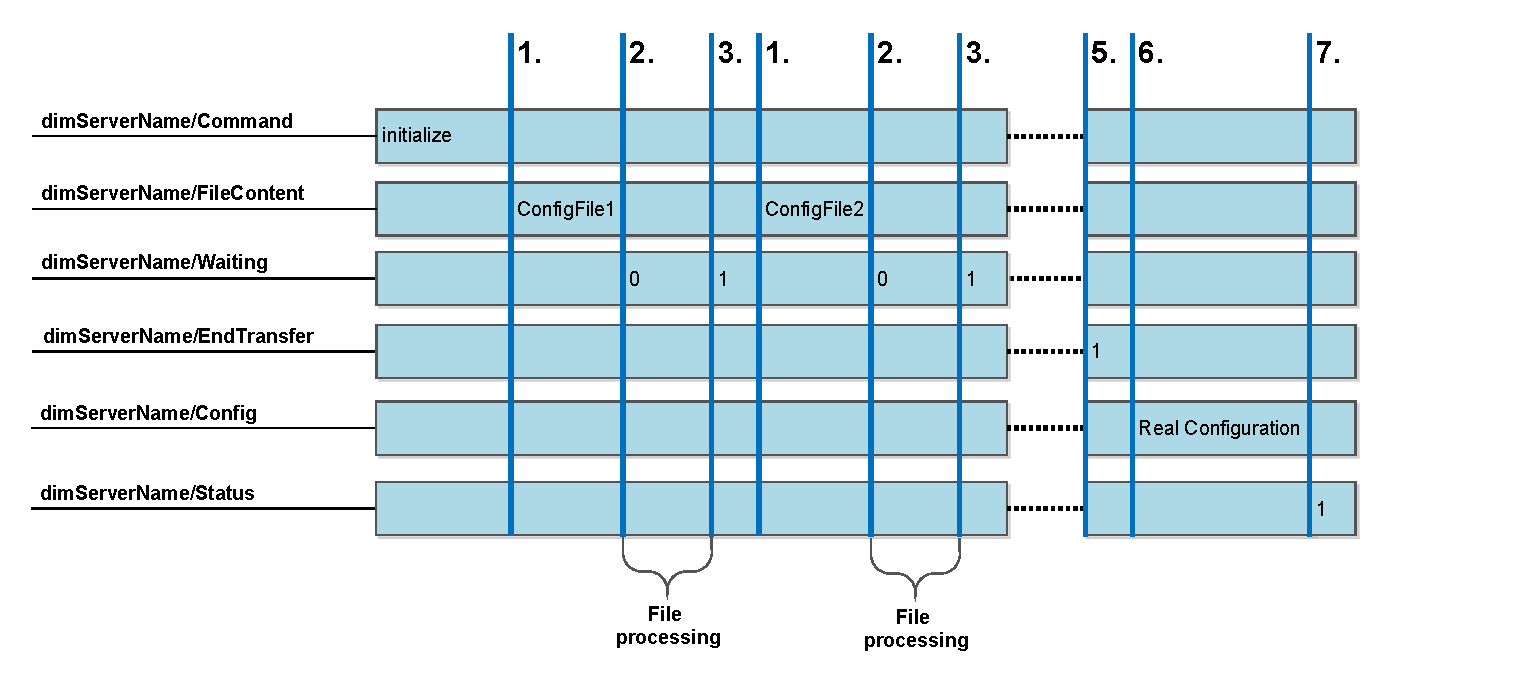
\includegraphics[width=\textwidth]{Doc/Configuration}
	\caption{Sketch of the procedure for the transfer of a configuration file from the RunControl to
	a device.}
	\label{fig:fileTransfer}
\end{figure}
The file transfer mechanism will work as depicted in Figure \ref{fig:fileTransfer} and explained in
details hereafter:
\begin{enumerate}
	\item \label{transf:start} After sending one of the commands described in \ref{sec:commands}, the
	RunControl will send the content of the first configuration file as a string on the command slot
	\ref{cmd:fileContent}. If no file has to be sent, the RunControl will move directly to point
	\ref{transf:end} of this procedure.
	\item Upon reception of the file content, the device sets the value of \ref{svc:waiting} to 0 and
	starts processing the configuration file (the details are left to the specific device
	implementation).
	\item \label{transf:wait} The RunControl wait until the device notifies that the file has been
	entirely processed and is waiting for further instructions by setting the value of
	\ref{svc:waiting} to 1.
	\item The RunControl repeats the points \ref{transf:start} and \ref{transf:wait} for the next
	configuration files until the last one has been processed.
	\item \label{transf:end} Once the entire configuration has been applied the RunControl sends 1 on
	\ref{cmd:endTransfer} to warn the device that there are no more configuration files.
	\item The device is now supposed to report back the current configuration. It will generate a file
	containing all the current parameter values, possibly in the same format as the configuration
	file. The file is transmitted to the RunControl by publishing it on the service port
	\ref{svc:config} and is stored in the offline database. Two possibilities are given to the
	subsystem:
	\begin{itemize}
		\item When applying the configuration files, keeping track of the real value of each parameter
		(the one that has been applied) and report this list of values, trusting that everything went
		well and that these values were effectively loaded in the hardware.
		\item Request the hardware for the actual value of each parameter and report this list of true
		values.
	\end{itemize}
	\item Finally the device updates its state parameters \ref{svc:state} or \ref{svc:stateParams},
	indicating the end of the configuration procedure. 
\end{enumerate}
At any point of the procedure, if something goes wrong or an anomaly is detected by the device, it
can move to an ERROR state that will interrupt the procedure. 

\section{Logging}\label{sec:logging}
The RunControl will be connected to three different databases: the configuration database containing
the recipes and the configuration files, the online database storing information related to the
run and the instantaneous state of the data taking, PC farm, \ldots and finally the offline
database that will contain the subset of the online values that are relevant to future analysis and
the configuration for each run. 

% Online and offline databases have different purposes. The online database is
% used by the RunControl as a real-time database while the offline database is
% used mostly for delayed reconstruction and analysis purposes. Their schemes are
% therefore different and the online database should not be loaded with the high
% read rates required by the offline database. Furthermore part of the values
% stored by the RunControl are not relevant to reconstruction and analysis jobs.

In addition to the run values logging, there will be a centralized device logging. This logging will
be displayed in the control room and recorded in the database. Every device will implement the
service port \ref{svc:logging} providing the source id, a severity code and the
text message itself. Four severity levels are allowed:
\begin{itemize}
  \item 0 for \textbf{Info}, an information that the user might want to know but
  no action is needed.
  \item 1 for \textbf{Warning}, an event has occurred and the user might want to
  take action even if it is not mandatory.
  \item 2 for \textbf{Error}, an event has occurred and the user should take
  action.
  \item 3 for \textbf{Fatal}, a fatal error has occurred and the run should be
  aborted.
\end{itemize}

\section{Alternative/Additional functionalities}
Alternative or additional functionalities can be provided by or to the device. Any of the
possibilities listed hereafter as well as anything not following the standards described
up to this point are to be discussed and agreed with the RunControl developers well in advance.

Alternative or additional services are given below and are taken from devices
already integrated in the RunControl. This is given as an example of services
that can be implemented beyond the minimum interface described in the previous
sections:
\begin{enumerate}[label=\textbf{ASVC.\arabic*}]
	\item \label{svc:stateParams} dimServerName/paramName: As stated in section
	\ref{sec:FSM} every device is described as a Finite State Machine in
	the RunControl. The proposed interface assumes that the device is internally
	following the same FSM diagram and keeping track of its current state,
	complying with the convention outlined in Table \ref{table:FSMStates}. On
	another hand the RunControl is able to determine itself in which state is the
	device if some requirements are met: the device provides a list of parameters
	and a set of rules are defined to infer the current state from these
	parameters.
	While the rules have to be given to the RunControl developers, the
	parameters values are read from a series of dim services, each service
	providing the value of a single parameter. This list of services is an
	alternative to the standard \ref{svc:state} and replaces it.
	\item dimServerName/TriggerNumber (Format: ``X:1''): This service is
	implemented by the current trigger processor. It provides the number of
	triggers generated during the current burst and is updated regularly during
	the burst.
\end{enumerate}

Again the additional command given below and are taken from devices already
integrated in the RunControl and given as an example of commands that can be
implemented beyond the minimum interface described in the previous sections:
\begin{enumerate}[label=\textbf{ACMD.\arabic*}]
	\item dimServerName/SendTrigger (Format: ``X:1''): This command is
	implemented by the current trigger processor. It requests the trigger processor
	to generate a certain number of triggers during next burst. This command has
	been created for testing and demonstration purposes during the commissioning of
	the TDAQ and will be disabled for normal runs.
\end{enumerate}

\section{Acknowledgment}
We would like to thank J.~Kunze, R.~Lietava and V.~Cerny for their contribution to the initial
implementations of the interface to the RunControl.

\appendix
\appendixpage
\section{Dim data format}\label{app:dimFormat}
%
A DIM service can contain different format of data: single value of a given
type, multiple values of a given type, structure with mixed types. This is
explained in the DIM documentation\cite{biblio:DIM}:

\textit{The available types are C(har), I(nt), L(ong), S(hort), D(ouble),
F(loat) or X(tra long). The format has to be specified as a description string in the form
``T:N;T:N;T:N'' where T is the type and N is the number of items of that type.
A data type alone at the end of string means all following items are of type T.}

In this document we use mostly the description ``I:1'' which means we are
transmitting a single integer and ``C'' which means a suite of chars (i.e. a
string).

\thebibliography{}

\bibitem{biblio:TEL62}{B. Angelucci et al., \textit{TEL62: an integrated trigger and data
acquisition board}, JINST 7 (2012) C02046.}
\bibitem{biblio:DIM}{http://dim.web.cern.ch/dim/}
\bibitem{biblio:TDAQNote}{M.S. Sozzi et al., \textit{NA62 online software and TDAQ interface.},
NA62 Note NA62-11-02, 2011}
\bibitem{biblio:JCOP}{https://j2eeps.cern.ch/wikis/display/EN/JCOP+Framework}
\end{document}
